\documentclass[10pt,a4paper]{article}
\usepackage[utf8]{inputenc}
\usepackage[T1]{fontenc}
\usepackage[french]{babel}
\usepackage{hyperref}
\usepackage{geometry}
\geometry{a4paper,margin=10mm,footskip=0mm}
%\setlength\leftmargin{2cm}
%\setlength\rightmargin{2cm}
\fontfamily{ppl}
\usepackage{graphicx}
\setlength\parindent{0pt}
\pagenumbering{gobble}
\frenchbsetup{StandardLists=true} % à inclure si on utilise \usepackage[french]{babel}
%\usepackage{enumitem}
\usepackage{amssymb}

\usepackage{soul}
\usepackage[svgnames]{xcolor}
\sethlcolor{LightYellow}
\newcommand{\grisclair}[1]{\colorbox{LightGray}{#1}}
\newcommand{\jaunepale}[1]{\colorbox{LightYellow}{#1}}
\newcommand{\bleupale}[1]{\colorbox{AliceBlue}{#1}}

\title{\bfseries{SoCo : Interface de suivi}}
%\author{Odile Bénassy}
\author{}
\date{}

\begin{document}
\pagestyle{empty}


\maketitle

%\emph{Toute utilisatrice autorisée peut créer ses propres formulaires SoCo.}

%\emph{À l'Université Paris Sud, il suffit pour cela de posséder un compte sur l'annuaire Adonis.}

\small{\emph{NB: Il est d'un usage de plus en plus répandu d'éviter de privilégier un genre plutôt qu'un autre. Toutefois, nous tenons à préserver la qualité de la langue. En conséquence, pour le présent document, nous adoptons la convention suivante : nous parlons d'un utilisateur - qui peut être aussi bien une utilisatrice bien évidemment - et d'une organisatrice - qui, de même, pourrait être aussi bien un organisateur.}}

\normalsize

\section*{\jaunepale{\emph{Visualisation des inscriptions}}}

\begin{itemize}
  \item Une fois sur le service, identifiez-vous et pénétrez dans l'\emph{espace réservé} (\url{https://soco.jm.u-psud.fr/suivi})
  \item Vous arrivez sur la page d'index du \emph{suivi}, qui reprend les colloques que vous devez suivre
  \item Choisissez le colloque sur lequel vous souhaitez travailler : la liste des inscriptions est là, sous forme de tableau
\end{itemize}

\begin{figure}[h]
  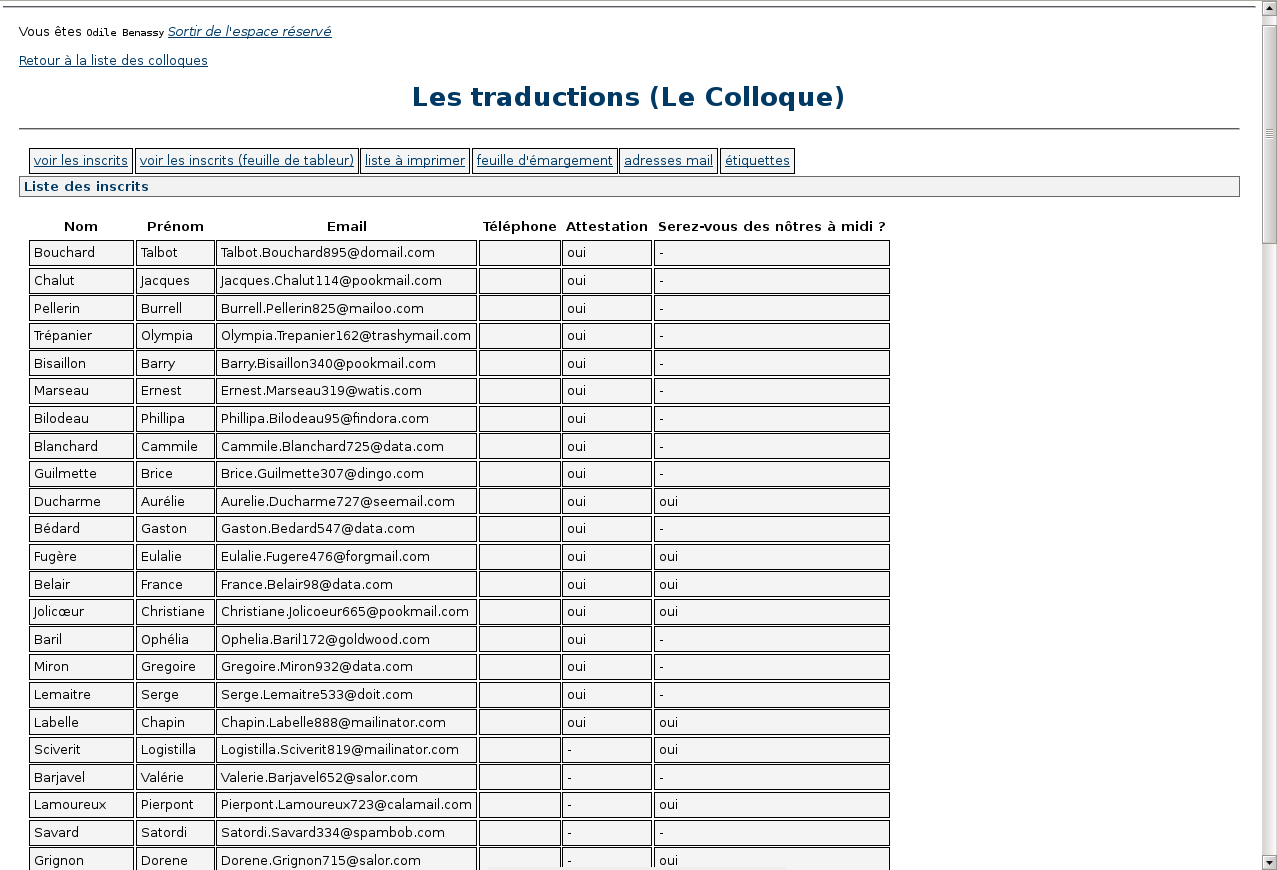
\includegraphics[width=500px]{images/suivi-colloque-3}
 \end{figure}

\section*{\jaunepale{\emph{Documents à télécharger}}}

Les différents petits onglets, sous le titre, sont autant de liens vers des documents à télécharger :

\begin{itemize}
  \item \emph{voir les inscrits} $\longrightarrow$ le tableau des inscrits que vous avez sous les yeux
  \item \emph{voir les inscrits (feuille de tableur)} $\longrightarrow$ le tableau des inscrits, au format CSV (pour tableur)
  \item \emph{liste à imprimer} $\longrightarrow$ la liste des inscrits : nom, prénom, institution, fonction
  \item \emph{feuille d'émargement} $\longrightarrow$ la liste d'émargement : nom, prénom, institution, case pour la signature
  \item \emph{envoi groupé} $\longrightarrow$ vous fournit toutes les adresses électroniques ; à copier-coller dans la fenêtre de composition quand vous voulez envoyer un courriel à tous les inscrits
  \item \emph{étiquettes} $\longrightarrow$ feuilles de badges à imprimer : format 92mm $\times$ 54mm, 9 étiquettes par page, avec logo et traits de coupe
\end{itemize}

\newpage

\section*{\jaunepale{\emph{Modification d'un formulaire}}}

La date de clôture des inscriptions se modifie très facilement, depuis la page d'index.

\begin{figure}[h]
  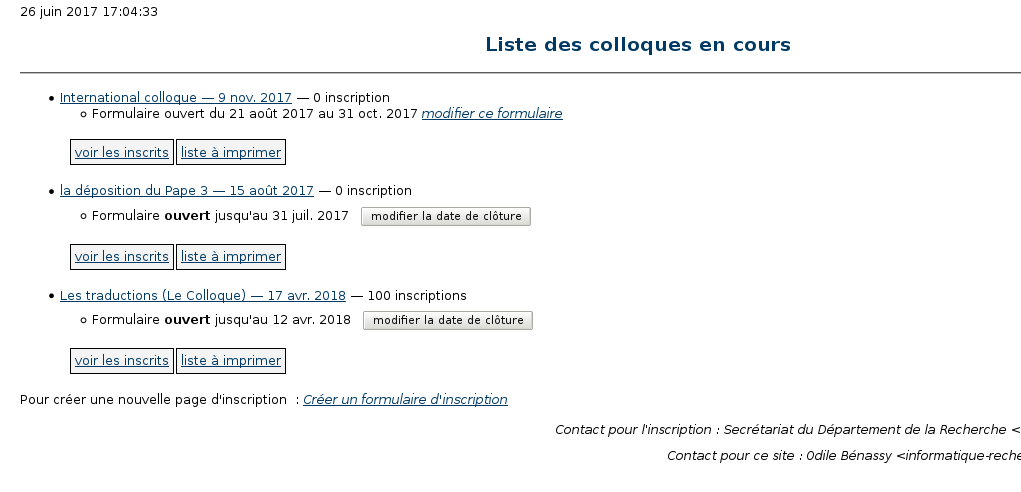
\includegraphics[width=500px]{images/suivi-index-2}
 \end{figure}

Pour tous les autres paramètres, il faut s'adresser aux organisatrices.

NB : pour des raisons de sécurité, les organisatrices du colloque sont tenues informées - par mail - de la modification de la date de clôture.

\section*{\jaunepale{\emph{Améliorations prévues}}}

Les améliorations suivantes feront partie d'une nouvelle version :

\begin{itemize}
  \item Réaction en fonction du nombre d'inscriptions par comparaison avec la capacité d'accueil : envoi de mail aux organisatrices, blocage...
  \item En plus de CSV, export dans les formats natifs des tableurs (Excel et LibreOffice)
  \item Amélioration de la page d'envoi groupé
\end{itemize}

 \fcolorbox{Black}{LightGray}{%
  \minipage[t]{\dimexpr0.9\linewidth-2\fboxsep-2\fboxrule\relax}
  \emph{Le logiciel SoCo a été réalisé, à l'\href{http://www.jm.u-psud.fr}{UFR Jean Monnet de l'Université Paris Sud}, par \href{mailto:odile.benassy@u-psud.fr}{Odile Bénassy}, responsable du service des systèmes d'information, en collaboration avec les responsables du service de la recherche du service de la communication. Ce logiciel prend la suite d'un autre, réalisé en 2007 par la même personne.}
  \endminipage}\hfill

%\fcolorbox{White}{White}{Fertig!}

\end{document}
